\documentclass[12pt,titlepage]{article}

\usepackage{tikz}
\usepackage{hyperref}

\title{Creating Figures With TikZ}
\author{Me}
\date{\today}

\begin{document}
\maketitle

\newpage
\thispagestyle{empty}
\tableofcontents
\newpage

\section{Introduction to TikZ}
\begin{itemize}
    \item \url{https://www.overleaf.com/learn/latex/TikZ_package}
    \item \url{https://ctan.org/pkg/pgf?lang=en}
\end{itemize}

\section{Drawing Lines}

First we have to include the TikZ package in the preamble with \verb|\usepackage{tikz}|.

The figure we want to draw has to be enclosed in the "tikzpicture" env.

In the figure \ref{tikz:1st_figure} below we are using the following code:
\begin{verbatim}
\begin{tikzpicture} 
    \draw (0, 0) -- (2, 0);
    \draw (2, 0) -- (1, 1.73205);
\end{tikzpicture} % \label{tikz:1st_figure}

To draw a line, where:
    (0, 0) => the starting point of the line,
    -- => the sign that the line is going from to,
    (2, 0) => the ending point of the line
    ; => to finish the TikZ input command
    

All the lengths are calculated in centimeters.

Instead of creating new \draw commands for each line we can also draw
them by simply adding another "-- (x, y)". Like this:

    \draw (0, 0) -- (2, 0) -- (1, 1.73205) -- (0, 0);

We can also use a "cycle" Instead of the "(0, 0)" point ro specify that
we are going right back to the beginning, like this:

    \draw (0, 0) -- (2, 0) -- (1, 1.73205) -- cycle;

It is preffered method of creating a closed shape as using the precise
point can create some random artefacts.
\end{verbatim}

\newpage

\begin{verbatim}
We can also change the size of the figure using the "scale" option, like:

    \begin{tikzpicture}[scale = 3]

We can also specify which axis we want to scale with: xscale / yscale.

There is also an option to make the lines thicker with option used in
\draw command:

    \draw[ultra thick]

Or change the line style:

    \draw[dashed] / [dotted]

If we want to draw more lines with the same style we can just separate the commands with space, like:
    \draw[dashed] (1, 0) -- (1, 1.73205) (0, 0) -- (1.5, 0.866)
        (2, 0) -- (0.5, 0.866);
We can also make the LaTeX calculate the lenghts for us by using
"{sqrt(3)}" Instead of the "1.73205".

To center the TikZ picture we use the "figure" env to wrap it in
and with that we can also use the [h] option to change its placement.
\end{verbatim}

\begin{figure}[h!]
    \centering
    \begin{tikzpicture}[scale = 3]
        \draw[ultra thick] (0, 0) -- (2, 0) -- (1, {sqrt(3)}) -- cycle;
        \draw[dashed] (1, 0) -- (1, 1.73205) (0, 0) -- (1.5, 0.866) (2, 0) -- (0.5, 0.866);
    \end{tikzpicture}
    \caption{This is my first TikZ figure and it is beautiful.}
    \label{tikz:1st_figure}
\end{figure}

\newpage
\section{Drawing Lines Exercise}

\begin{figure}[h]
    \centering
    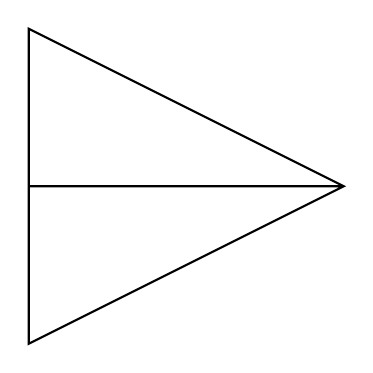
\begin{tikzpicture}[scale=2]
        \draw[thick] (0, 0) -- (0, 2) -- (2, 1) -- cycle (0, 1) -- (2, 1);
    \end{tikzpicture}
    \caption{This is the 2nd TikZ figure!}
\end{figure}

Code used:
\begin{verbatim}
\begin{figure}[h]
    \centering
    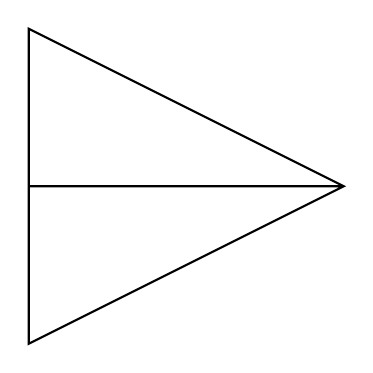
\begin{tikzpicture}[scale=2]
        \draw[thick] (0, 0) -- (0, 2) -- (2, 1) -- cycle (0, 1) -- (2, 1);
    \end{tikzpicture}
    \caption{This is the 2nd TikZ figure!}
\end{figure}
\end{verbatim}

\newpage
\section{Basic Shapes}

\begin{verbatim}
To write the rectangle we specify the lower left corner and upper right
corner and connect them with "rectangle" instead of the "--" as we did before.
Like this:
    \draw[thick] (-3, -3) rectangle (3, 3);

We can also draw circles, where we specify the center point of the circle
and then connect it with options using "circle":
    \draw[thick] (0, 0) circle [radius = 3];
The option bracket can take more parameters than just a radius. We can also specify the draw color the same way as we did with the thickness:
    \draw[thick, red] (0, 0) circle [radius = 3];

To fill in the shape we can do it in 2 different ways - option or command:
    \draw[fill, green] (0, 0) circle [radius = 0.1];
    OR
    \fill[blue] (0, 0) circle [radius = 0.1];

We can specify the density of the dots / dashes with the "densely" or "loosely":
    \draw[ultra thick, blue, loosely dotted] (0, 0) -- (3, 0);

We can place text in the figures:
    \node[above] at (0, 0.1) {The center.};
    where:
        above => option specifying the placement relative to the point and
                    below, left, right can also be used,
        at (0, 0) => the point at which we want the text to be,
        {Text} => the caption we want to be displayed.

To use a caption which is long and needs the line break ("\\"),
we have to add another option, which is "align":
    \node[below, align = left] at (1.5, 0) {The radius of \\
                                            the circle is 3.};
\end{verbatim}

\begin{figure}[h]
    \centering
    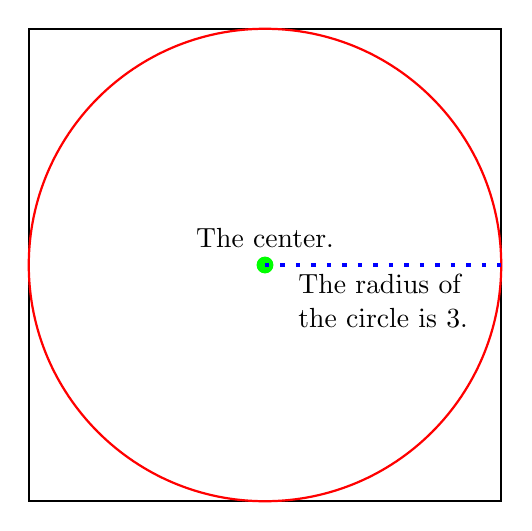
\begin{tikzpicture}[scale=1]
        \draw[thick] (-3, -3) rectangle (3, 3);
        \draw[thick, red] (0, 0) circle [radius = 3];
        \draw[fill, green] (0, 0) circle [radius = 0.1];
        % \fill[blue] (0, 0) circle [radius = 0.1];
        \draw[ultra thick, blue, loosely dotted] (0, 0) -- (3, 0);
        \node[above] at (0, 0.1) {The center.};
        \node[below, align = left] at (1.5, 0) {The radius of \\ the circle is 3.};
    \end{tikzpicture}
    \caption{Here comes the 3rd figure. This one is more complicated!}
\end{figure}

\newpage
\section{Basic Shapes Exercise}

\begin{figure}[h]
    \centering
    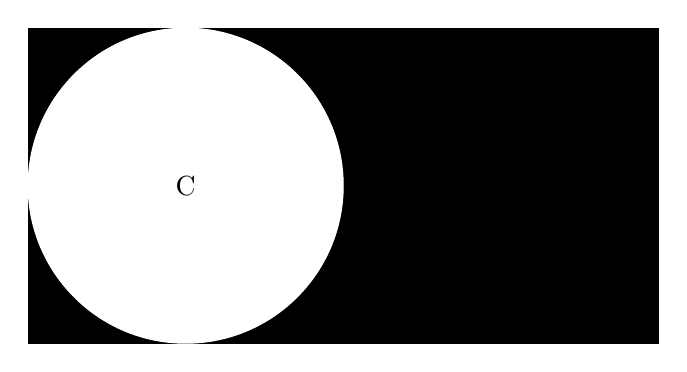
\begin{tikzpicture}[scale=1]
        \draw[fill] (-3, -2) rectangle (5, 2);
        \draw[white, fill] (-1, 0) circle [radius = 2];
        \node at (-1, 0) {C};
    \end{tikzpicture}
    \caption{This is the 4th figure. Yay!}
\end{figure}

\newpage
\section{Plotting Functions}

\begin{verbatim}
To draw a plot, we first have to draw the axis:
    \draw[->] (-0.1, 0) -- (10, 0); => the X axis
    \draw[->] (0, -0.1) -- (0, 5); => the Y axis
        The "->" option creates the arrow head of the axis

When we have the axis we can create the grid:
    \draw[gray, ultra thin] (-0.1, -0.1) grid (9.9, 4.9);
The 9.9 & 4.9 makes the grid without the last lines on right and at the top

Now to plot a Function we use:
    \draw[] plot (\x, \x/2);
BUT this will not work as we think it should. We have to specify the domain
of the function to make the plot fit in the grid we created:
    \draw[domain=0:9.9] plot (\x, \x/2);
BUT (2nd!) if we have more Functions with the same domain we can specify it
in the tikzpicture option.

Now that we have the Functions ploted we can label them. We do that by modifying
the draw command to include the node (same as we did with multiple lines):
    \draw[orange, thick] plot (\x, \x/2) node[above] {$f(x) = \frac{x}{2}$};
\end{verbatim}
\begin{figure}[h]
    \centering
    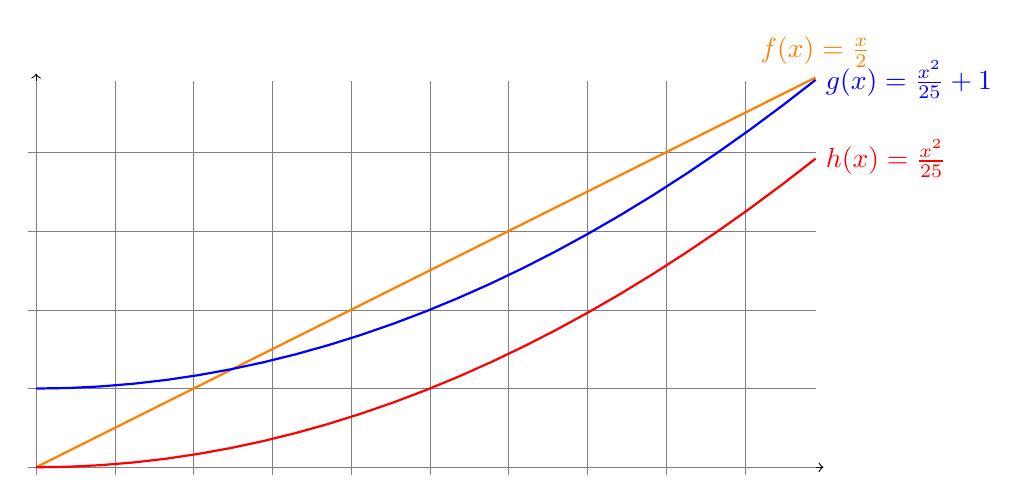
\begin{tikzpicture}[domain=0:9.9]
        \draw[->] (-0.1, 0) -- (10, 0);
        \draw[->] (0, -0.1) -- (0, 5);
        \draw[gray, ultra thin] (-0.1, -0.1) grid (9.9, 4.9);

        \draw[orange, thick] plot (\x, \x/2) node[above] {$f(x) = \frac{x}{2}$};
        \draw[blue, thick] plot (\x, \x * \x / 25 + 1) node[right] {$g(x) = \frac{x^{2}}{25} + 1$};
        \draw[red, thick] plot (\x, {pow(\x, 2) / 25}) node[right] {$h(x) = \frac{x^{2}}{25}$};
    \end{tikzpicture}
    \caption{This is getting serious!}
\end{figure}

\newpage
\section{Plotting Functions Exercise}

\begin{figure}[h]
    \centering
    \begin{tikzpicture}[domain=-1.5:1.5]
        \draw[->] (-1.6, 0) -- (1.6, 0);
        \draw[->] (0, -0.1) -- (0, 5);
        \draw[brown] plot (\x, {exp(\x)}) node[right] {$\exp(x)$};
    \end{tikzpicture}
    \caption{The exponential function denoted exp(\textbackslash x) plotted from -1.5 to 1.5. We have used the color brown to color the graph}
\end{figure}

\newpage
\section{Plotting Curves}
To note that the argument x of the cos function is in radians instead of the degrees we write it as \verb|cos(\x r)|. The code:
\begin{verbatim}
    \draw[->] (0, -2.7) -- (0, 2.7);
    \draw[->] (-4.5, 0) -- (1.1, 0);
    \draw[gray, ultra thin] (-4.5, -2.6) grid (0.9, 2.5);

    \draw[domain=0:2*pi, smooth, pink, thick] plot ({2*(1-cos(\x r))
        * cos(\x r)}, {2*(1-cos(\x r)) * sin(\x r)});
    % 2*pi/3
    \draw[loosely dotted, thick] (0, 0) -- ({2*(1-cos(2*pi/3 r))
        * cos(2*pi/3 r)}, {2*(1-cos(2*pi/3 r)) * sin(2*pi/3 r)})
        node[above] {$\frac{3}{2} (-1, \sqrt{3})$};
    \draw[fill] ({2*(1-cos(2*pi/3 r)) * cos(2*pi/3 r)},
        {2*(1-cos(2*pi/3 r)) * sin(2*pi/3 r)}) circle [radius = 0.05];
    \draw[thick, dotted] ({2*(1-cos(2*pi/3 r)) * cos(2*pi/3 r)},
        {2*(1-cos(2*pi/3 r)) * sin(2*pi/3 r)})
        -- (-3/2, 0) node[below] {$-\frac{3}{2}$};
\end{verbatim}
\begin{figure}[h]
    \centering
    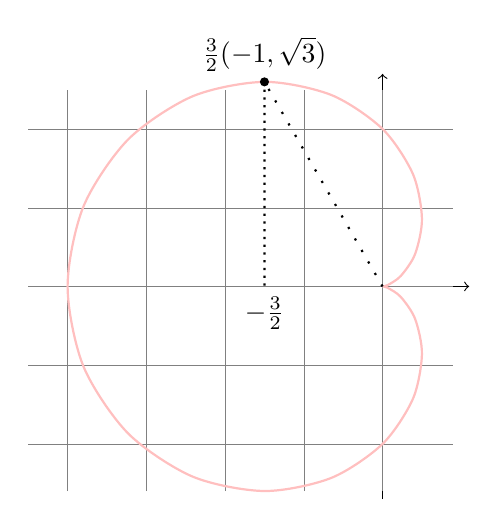
\begin{tikzpicture}
        \draw[->] (0, -2.7) -- (0, 2.7);
        \draw[->] (-4.5, 0) -- (1.1, 0);
        \draw[gray, ultra thin] (-4.5, -2.6) grid (0.9, 2.5);

        \draw[domain=0:2*pi, smooth, pink, thick] plot ({2*(1-cos(\x r)) * cos(\x r)}, {2*(1-cos(\x r)) * sin(\x r)});
        % 2*pi/3
        \draw[loosely dotted, thick] (0, 0) -- ({2*(1-cos(2*pi/3 r)) * cos(2*pi/3 r)}, {2*(1-cos(2*pi/3 r)) * sin(2*pi/3 r)}) node[above] {$\frac{3}{2} (-1, \sqrt{3})$};
        \draw[fill] ({2*(1-cos(2*pi/3 r)) * cos(2*pi/3 r)}, {2*(1-cos(2*pi/3 r)) * sin(2*pi/3 r)}) circle [radius = 0.05];
        \draw[thick, dotted] ({2*(1-cos(2*pi/3 r)) * cos(2*pi/3 r)}, {2*(1-cos(2*pi/3 r)) * sin(2*pi/3 r)}) -- (-3/2, 0) node[below] {$-\frac{3}{2}$};
    \end{tikzpicture}
    \caption{The cardioid $\left(2(1-\cos(\theta))\cos(\theta),{2(1-\cos(\theta))\sin(\theta)}\right)$.}
\end{figure}

\end{document} 